%%%%%%%%%%%%%%%%%%%%%%%%%%%%%%%%%%%%%%%%%%%%%%%%%%%%%%%%%%%%%%%%%%%%%%
%%                    Non-Interaction
%%%%%%%%%%%%%%%%%%%%%%%%%%%%%%%%%%%%%%%%%%%%%%%%%%%%%%%%%%%%%%%%%%%%%%
\color{red}

\subsubsection{Glyph: \glyph{Non-Interaction}}\label{sec:non-interaction}

\glyph{Non-interaction} represents the absence of an interaction between two or more \glyph{entities} or \glyph{outcomes}, whether a non-covalent physical interaction, or a functional interaction, e.g. genetic interaction. Each arrowhead points to an interactor involved in the absent interaction. The result of the non-interaction is represented by \glyph{outcomes} (see section \ref{sec:outcome}), that is by filled dots on the line linking the two arrowheads in the case of a binary interaction, on a circle linked to the edges coming from the arrowheads in the case of a  n-ary interactions. The result of an interaction can be represented by any number of \glyph{outcomes}.

\begin{glyphDescription}
 \glyphSboTerm SBO:NEW
 \glyphOrigin Any \glyph{interactor} (\sect{interactors}).
 \glyphTarget Any \glyph{interactor} (\sect{interactors}).
 \glyphEndPoint Both origin and target extremities of a \glyph{non-interaction} carry an harpoon arrowhead. In the case of n-ary non-interactions, the arrows pointing to the \glyph{interactors} originate from a circle. 
 \glyphAux A \glyph{unit of information} containing a \glyph{cardinality} (\sect{miscellaneous-cv}) indicates the number of instances of an entity involved in an interaction. A \glyph{unit of information} on a binary non-interaction involving only one entity carrying the mention \glyph{cis} or \glyph{trans} precises if this is an absence of an intra-molecular interaction or and interaction between different instances of the same entity.
 \end{glyphDescription}

\begin{figure}[H]
  \centering
  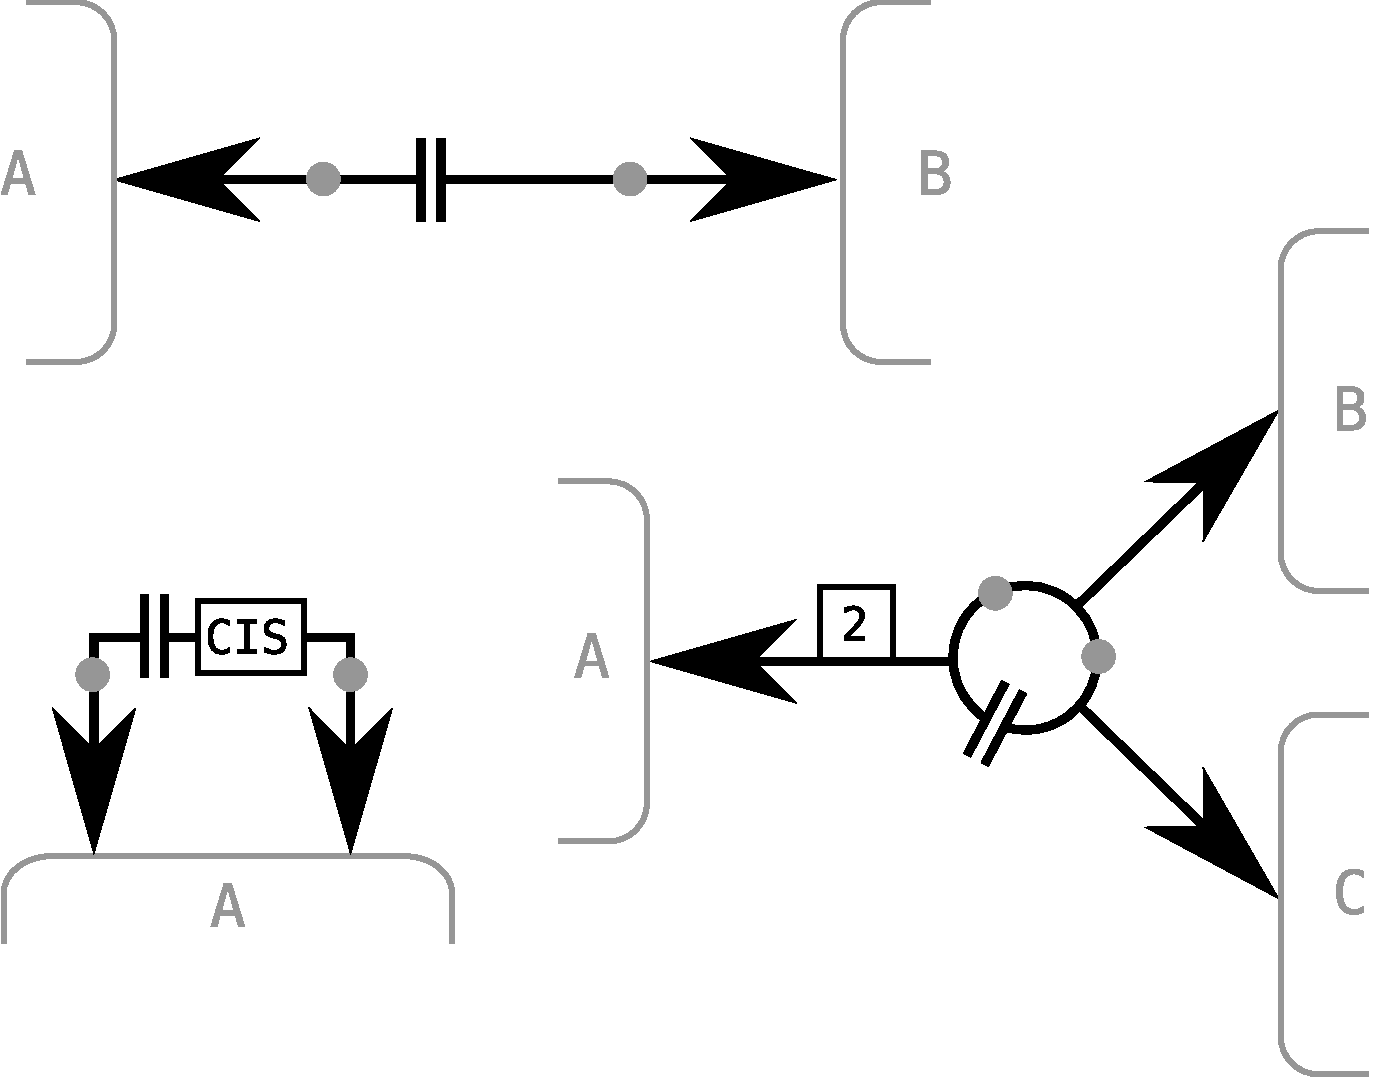
\includegraphics[scale = 0.3]{images/non-interaction}
  \caption{The \ER glyph for \glyph{non-interaction}. Top, binary non-interaction between two entities; bottom left, absence of an intra-molecular interaction; bottom right, absence of an n-ary interaction.}
  \label{fig:non-interaction}
\end{figure}

\normalcolor